\documentclass[10pt]{article}
\usepackage{fontspec}
\usepackage{polyglossia}
\setdefaultlanguage{french}
\usepackage[a4paper,margin=2.5cm]{geometry}
\usepackage{url,hyperref}
\usepackage{siunitx}
\usepackage{schemabloc}
\usepackage{listings}
\usepackage{auto-pst-pdf}
\usepackage{pst-circ}
\usepackage{soul}
\usepackage{verbatim}
\usepackage{lmodern}
\usepackage{tikz}
\usepackage[european,cuteinductors,siunitx]{circuitikz}
\usepackage{xunicode,xltxtra}
\usepackage{graphicx}
\usepackage{amsmath}
\usepackage{minted}
\usepackage{multicol}
\title{
\includegraphics{../../../images/inp-enseeiht} \\ ~ \\ ~ \\ ~ \\ ~ \\BE Lignes de transmissions}
\author{Ken Hasselmann, Guilhem Saurel}
\date{\today}
\begin{document}

 \begin{titlepage}
  \maketitle
  \tableofcontents
 \end{titlepage}

  \section{Parametre S et abaque de Smith}
   Valeur normalisée de l’impédance : $z_L=\cfrac{Z_L}{Z_0}=\cfrac{80 + j 5 \cdot 10^{-9} \cdot 2 \pi 2 \cdot 10^9}{50} = 1.6+i1.26$

   Coefficient de réflexion correspondant : $\Gamma = \cfrac{z_L-1}{z_L+1}=0.38+i0.30$

   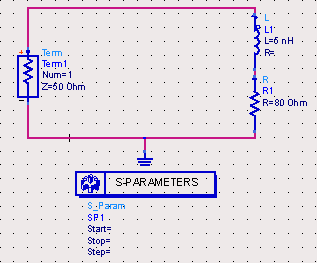
\includegraphics[width=8cm]{I2_a_circuit.PNG}
   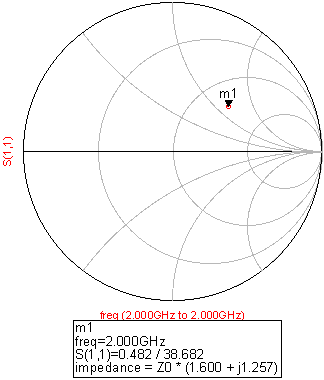
\includegraphics[width=8cm]{I2_a_smith.PNG}

   \newpage

   Lorsque l’on ajoute une ligne de transmission entre la source et la charge, on obtient une impédance ramenée au niveau du port d’entrée de $z_E = \cfrac{z_L +j \tan{\beta d}}{1 + j z_L \tan{\beta d}}=\cfrac{z_L +j \tan{E}}{1 + j z_L \tan{E}}$

   Le coefficient de réflexion correspondant est : $\Gamma=\cfrac{z_E-1}{z_E+1}$

   Dans le cas particulier d’une ligne quart d’onde, ceci donne $-0.38-i0.30$

   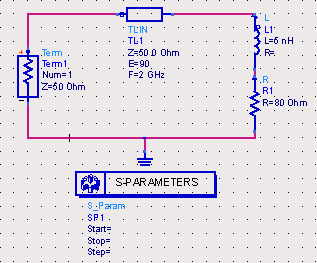
\includegraphics[width=8cm]{I2_b_circuit.PNG}
   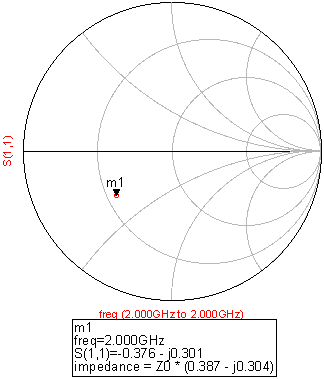
\includegraphics[width=8cm]{I2_b_smith.PNG}

   En utilisant l’outil «Tune», on peut modifier la longueur de la ligne en temps réel et voir le point se déplacer sur l’abaque de smith (ce qui peut être utile pour des réglages) :

   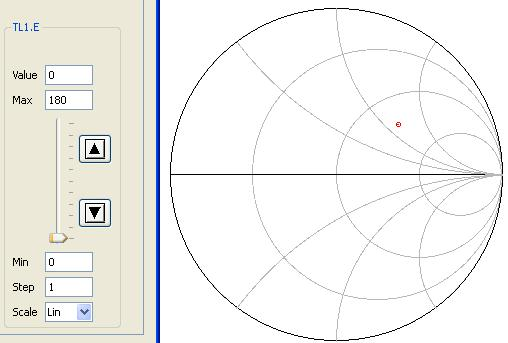
\includegraphics[width=8cm]{I2_c-0.jpg}
   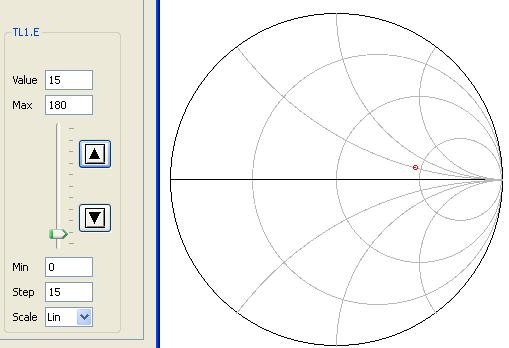
\includegraphics[width=8cm]{I2_c-15.jpg}
   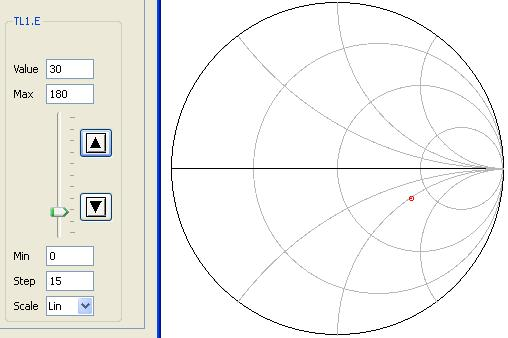
\includegraphics[width=8cm]{I2_c-30.jpg}
   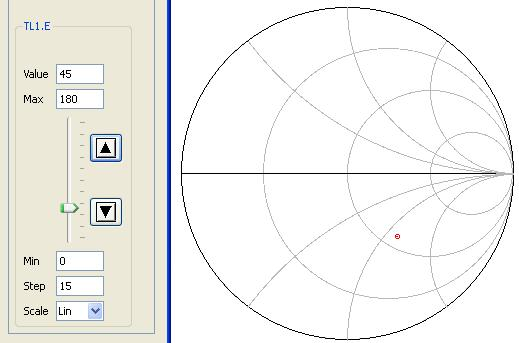
\includegraphics[width=8cm]{I2_c-45.jpg}

   %TODO : Quel est le lieu des impédances ramenées dans le plan de la source ?

   \newpage
   Cependant, on ne voit les points que un par un…

   On peut donc utiliser le «sweep parameter», qui permet sur la même abaque de voir tous les points :
   
   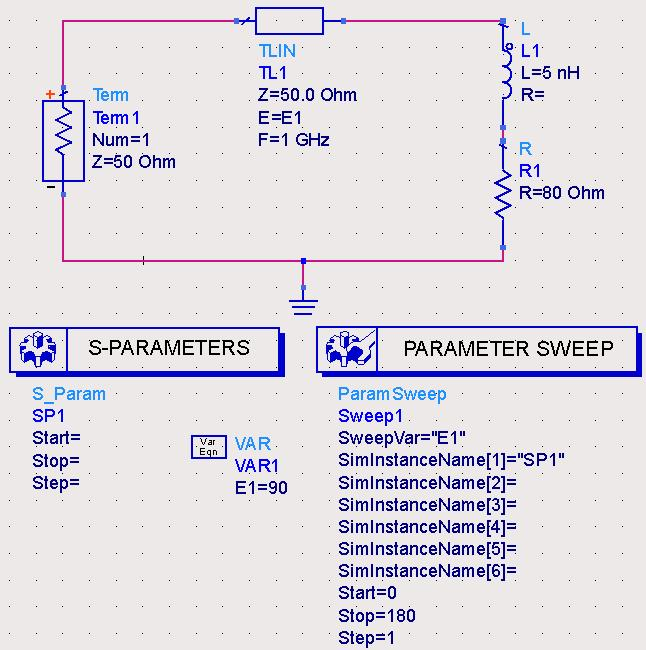
\includegraphics[width=8cm]{I2_d_circuit.jpg}
   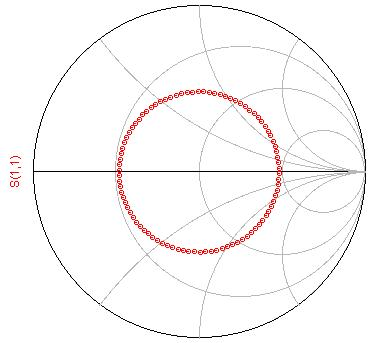
\includegraphics[width=8cm]{I2_d_simulation.jpg}

   Lorsque l’on enlève la bobine afin de ne garder que la partie réele de la charge, l’impédance ramenée dans le plan du port est donc la partie réele de celle que nous avions précédement : $z_L=\cfrac{Z_L}{Z_0}=\cfrac{80}{50} = 1.6$ ; ce que l’on vérifie sous ADS :

   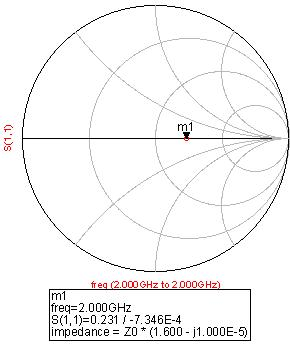
\includegraphics[width=8cm]{I2_e_impedance.jpg}

   \newpage
   On cherche maintenant à déterminer l’impédance de ligne $Z_C$ permettant d’obtenir une impédance ramenée $Z_E$ de $50 \Omega$ :
   
   $Z_E = Z_C \cfrac{Z_L +j Z_C\tan{\beta d}}{Z_C + j Z_L \tan{\beta d}} \simeq Z_C \cfrac{j Z_C \tan{E}}{j Z_L \tan{E}} \simeq \cfrac{Z_C^2}{Z_U}$, 

   Donc pour $Z_E=50 \Omega$, on a $Z_C=\sqrt{Z_E Z_L} = 63,25 \Omega$

   On vérifie la position du point sur ADS :

   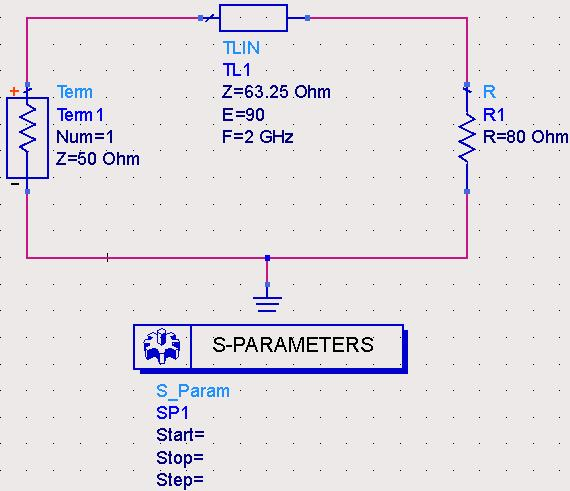
\includegraphics[width=8cm]{I2_e_50-circuit.jpg}
   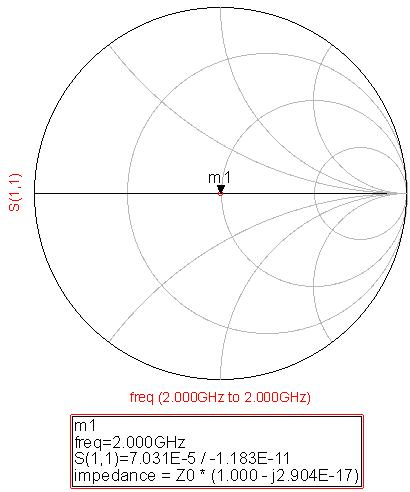
\includegraphics[width=8cm]{I2_e_50-simulation.jpg}

   On peut visualiser le lieu des charges ramenées en fonction des impédances de la ligne, avec un «sweep parameter» :

   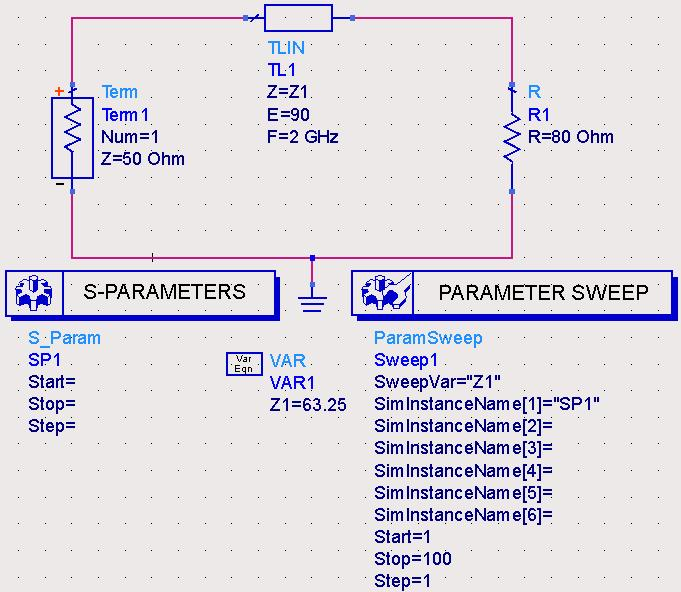
\includegraphics[width=8cm]{I2_e_impedances-circuit.jpg}
   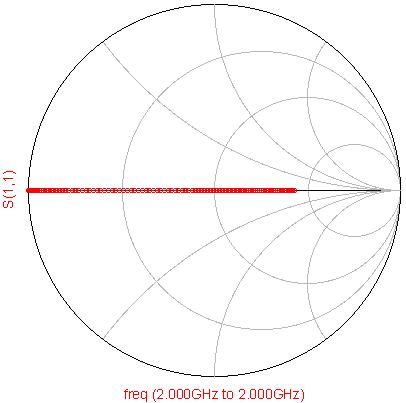
\includegraphics[width=8cm]{I2_e_impedances-simulation.jpg}

   \newpage
   Si l’on trace le coefficient de réflexion en fonction de la fréquence pour une impédance de ligne permettant de rammener $50 \Omega$, on remarque que celui-ci est effectivement très faible pour 2GHz.
   
   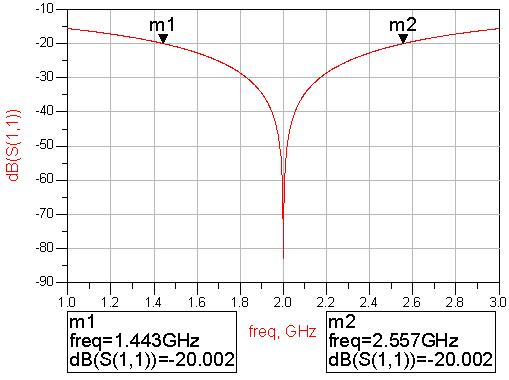
\includegraphics[width=8cm]{I2_e_bode.jpg}

   On mesure comme fréquences de coupure 1443 Hz et 2557 Hz, d’où une bande passante de 1114 Hz.

   %TODO calculer le ROS

   Pour calculer l’impédance ramenée par une ligne de longueur quelconque chargée par un court-circuit, on pose $Z_u = 0$, d’où $Z_R = \cfrac{j Z_c \tan{E}}{Z_c} \Rightarrow Z_R = \infty$

   De même, pour un circuit ouvert, $Z_u = \infty$, d’où $Z_R = 0$.

 \section{Matrices Chaines, comportement fréquentiel}
  \begin{center}
  \begin{pspicture}(7,3)
   \pnode(1,2.5){A}
   \pnode(1,0.5){B}
   \pnode(5,2.5){C}
   \pnode(5,0.5){D}
   \pnode(0,2.5){a}
   \pnode(0,0.5){b}
   \pnode(6,2.5){c}
   \pnode(6,0.5){d}
   \quadripole(A)(B)(C)(D){ABCD}
   \tension(B)(A){$V_1$}
   \tension[labeloffset=-0.5](D)(C){$V_2$}
   \wire[intensitylabel=$I_1$](a)(A)
   \wire(b)(B)
   \wire[intensitylabel=$I_2$,intensitylabeloffset=-0.5](c)(C)
   \wire(d)(D)
  \end{pspicture}
  \[
   \begin{pmatrix}
    V_1 \\
    I_1
   \end{pmatrix}
   =
   \begin{pmatrix}
    A & B \\
    C & D
   \end{pmatrix}
   \begin{pmatrix}
    V_2 \\
    -I_2  
   \end{pmatrix}
  \]
  \end{center}
  d’où

  $V _1 = A V_2 - B I_2$

  $I_1 = C V_2 - D I_2$

  On en déduit :
  \[ ABCD =
  \begin{pmatrix}
   1 & 0 \\
   \cfrac{1}{j Z_c \tan{\beta d}} & 1
  \end{pmatrix}
  \]

  On peut voir ceci sous ADS pour des fréquences comprises entr 0.1 GHz et 5 GHz, que ce soit en entrant la matrice :

  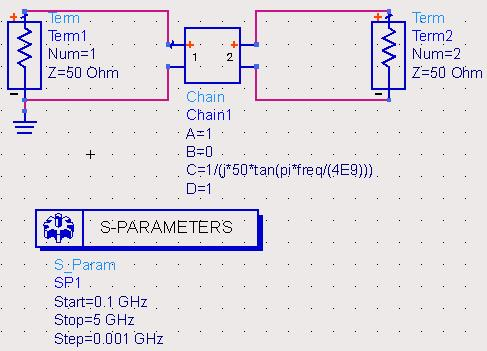
\includegraphics[width=8cm]{I3_b_circ.jpg}
  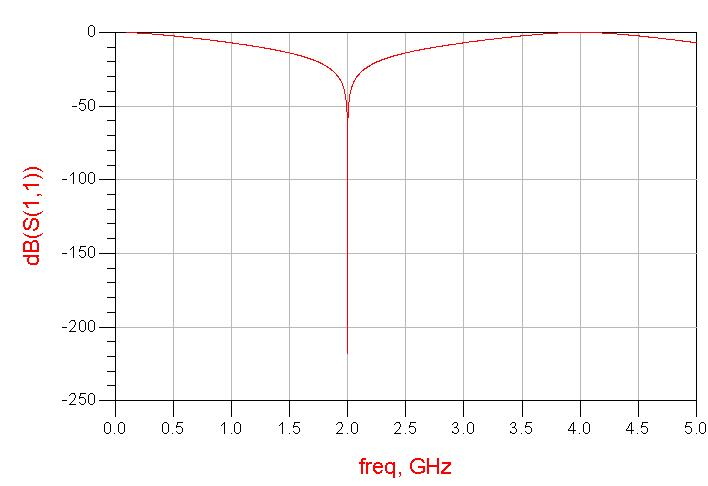
\includegraphics[width=8cm]{I3_b_simu.jpg}

  Ou en mettant directement un stub :

  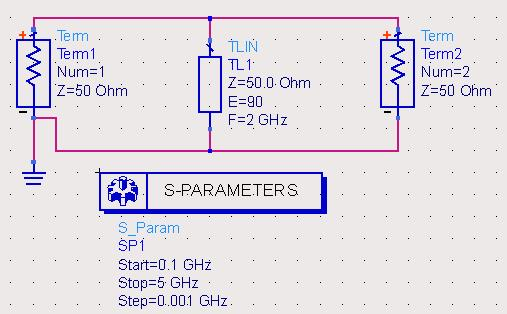
\includegraphics[width=8cm]{I3_b_circ_stub.jpg}
  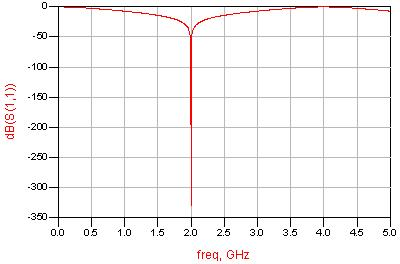
\includegraphics[width=8cm]{I3_b_simu_stub.jpg}

  Sur cette même gamme de fréquence, on peut faire varier la longuer électrique de la ligne entre 45° et 135°, que ce soit en changeant directement E ou en modifiant la longueur physique des stubs :

  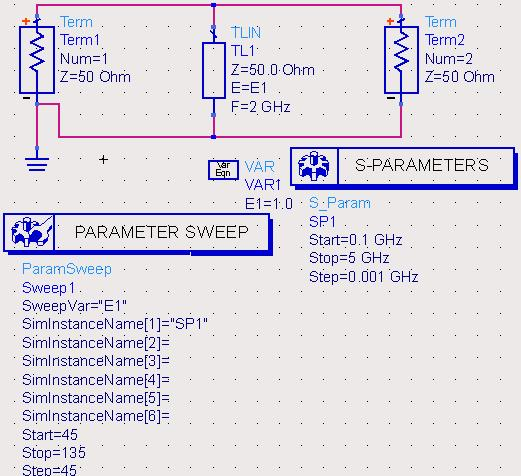
\includegraphics[width=8cm]{I3_c_circ.jpg}
  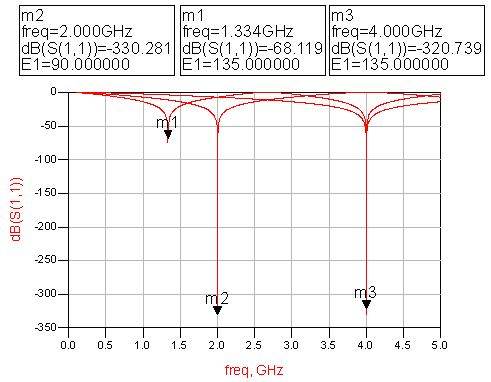
\includegraphics[width=8cm]{I3_c_simu.jpg}

 \section{Annexes}
  Voici le fichier Scilab contenant tous les calculs :
  \inputminted[linenos]{matlab}{calculs.sci}

\end{document}
